From the discussion in chapter \ref{TH_intro} it is evident that with the integration of DERs in the grid several new challenges are coming into light. To help in the integration of DERs and combat these challenges ADMS and DERMS are being developed. Two significant components of DERMS are voltage regulation and energy management. This chapter focuses on the state of the art research on these two topics. Analysis of research gaps in the areas and novel contribution of the research are also presented. 
\section{Voltage Regulation}
As mentioned in chapter \ref{TH_intro} voltage regulation is one of the primary challenges to be overcome in order to have a high penetration of DERs in the grid. Currently, there are two types of regulation devices available in the system. The first type is the traditional regulation devices (on load tap changers, switched capacitor banks, step voltage regulators) and the other types are power electronics based regulation devices (DG inverters and distribution static VAR compensators). There needs to be an optimum operation of both to reliably and cost-effectively maintain the voltage at all the nodes of the system. In literature, this problem is defined in two ways. It can be defined as an Optimum voltage regulation problem, or it can be defined as an optimum reactive power dispatch problem. Many alternative methods with different controllable components have been discussed in the literature to solve the problem. The following is a brief discussion of the controllable components which may be used to solve the problem \cite{VC_1}. 
\begin{itemize}
    \item \textbf{Generation curtailment during low demand:} The DGs generation may be curtailed during low demand periods to maintain the system voltage. This would be harmful to the DG owner because the DGs cannot operate in peak condition.
    \item \textbf{Reactive power control (VAR compensation) by reactive compensator:} Reactive VAR compensators placed at strategic points of the system can be used to absorb or inject reactive power.  
    \item \textbf{Area based OLTC (on load tap changer) coordinated voltage control:} The OLTC at the substation can be controlled to maintain voltage.
    \item \textbf{Inverters at DG sites:} The inverters of the DGs can be used similarly to the VAR compensators to inject reactive power or absorb reactive power as needed.
    \item \textbf{Energy storage:} If there are energy storage in the system their charging and discharging operations can be controlled to maintain system voltage.
\end{itemize}

Control methodologies which take into account all the components are a contemporary research topic and they can be divided into two main categories. 
\begin{enumerate}
    \item Centralized control
    \item Decentralized and distributed control
\end{enumerate}

\subsection{Centralized Control}
In this control strategy, every component of the distribution system is controlled from a centralized controller. Proper implementation of these methods requires a robust communication network in the distribution system. The centralized control methods considered here focus on control algorithms that make use of the DG inverters to maintain global voltage. 

An objective function to minimize active power loss in distribution network has been considered in \cite{CE_VC_1}. Reference \cite{CE_VC_2} focuses on reactive power control with an objective of minimizing voltage deviation at each bus according to a reference voltage. In \cite{CE_VC_3} the distribution network has been divided into different subsections to reduce the optimization complexity. In \cite{CE_VC_4} tap operation and system losses in radial distribution network were minimized by coordinating OLTCs and SVCs (static VAR compensators). In \cite{CE_VC_5} the day ahead prediction of DGs were used to aid in the regulation method. A real-time optimum control strategy with vehicle to grid interface is proposed in \cite{CE_VC_6}. Another control strategy utilizing energy storage systems and OLTCS is proposed in \cite{CE_VC_7}.

A centralized control strategy can provide the best performance possible, but it may not be the best solution for the future grid for the following reasons \cite{VC_1}:
\begin{itemize}
    \item They require significant investment in communication assets.
    \item A large number of small scale devices need to be controlled.
    \item There is an increased amount of uncertainty due to faults, electric vehicles, storage units, dynamic loads, variable DGs, restoration, reconfiguration etc.
    \item Increased computation complexity due to a large number of variables.
    \item Does not incorporate plug and play capabilities.
\end{itemize}

\subsection{Decentralized and Distributed Control}
Decentralized and distributed control schemes do not have a centralized hub where the control actions are calculated. They consist of multiple controllers which communicate with each other to maintain system stability \cite{DB_VC_1}.  Different decentralized and distributed control schemes are briefly discussed below.

\begin{itemize}
    \item \textbf{Distributed optimization method:} The optimum voltage control problem can be formulated as a non-convex optimal power flow problem. In these methods, some form of convex relaxation is applied to make the problem convex. Then the centralized convex problem is decomposed to and solved by distributed algorithms \cite{Kyrue}. References  \cite{KUt17,BAR16,BAR161,WZh16} are some of the recent literature using various distributed optimization methods to solve the voltage regulation problem.
    \item \textbf{Decentralized Methods:} In the decentralized method, each area solves its own voltage regulation problem and the solution only affects that area. Both heuristic methods and optimization methods may be used to solve the problems \cite{Kyrue}. \cite{MChss,MBa,XZh16,MNa16,LRe15,EDass} are some recent publications on this method.
    \item \textbf{Distributed Cooperation:} In this scheme, the secondary centralized control interacts with autonomous primary control. This results in a secondary control scheme that substitutes local control \cite{Kyrue}. References \cite{ABi13,FGu15,SAn13,QSh14} are some modern research on this topic.
    \item \textbf{Distributed Adaptive Control:} These methods monitor their performance and self-tunes its input value rather than maintaining a reference value. In \cite{ABi14} the adaptive secondary voltage control is formulated as a tracking synchronization problem. Neural networks were used to model the non-linear inverter dynamics \cite{Kyrue}.
    \item \textbf{Distributed Model Predictive Control:} In this method, the controllers predict their state over a finite time-horizon by gathering information from their neighbors and using the model of the system. In \cite{GLoss} model predictive control is used to minimize the voltage deviation until all the voltages synchronize to a reference value \cite{Kyrue}.
    \item \textbf{Decision Making:} In this method when there is a conflict between multiple objectives a decision maker is used to identify the solution \cite{Kyrue}. Expert-based decision makers are incorporated in smart agents in \cite{HEF12, HEF13}. The agents communicate using a contract net protocol option. The controllers in \cite{MEC13} exchange their constraints to solve a dynamic optimal dispatch problem.
    \item \textbf{Hybrid Methods:} In this case, the distributed control takes over when the local control fails to maintain the system voltage \cite{Kyrue}. Reference \cite{GMo13,YWa16} uses consensus algorithms for distributed control after local control fails. Reference \cite{DRe13} does active curtailment of DG units. In \cite{BAR13} the distributed control requests reactive power compensation from neighboring zones if voltage imbalance cannot be mitigated.
\end{itemize}
An overview of the advantages and disadvantages of the methods mentioned is given in Fig. \ref{fig:DIS_CVC}.
\begin{figure}[!h]
\centering
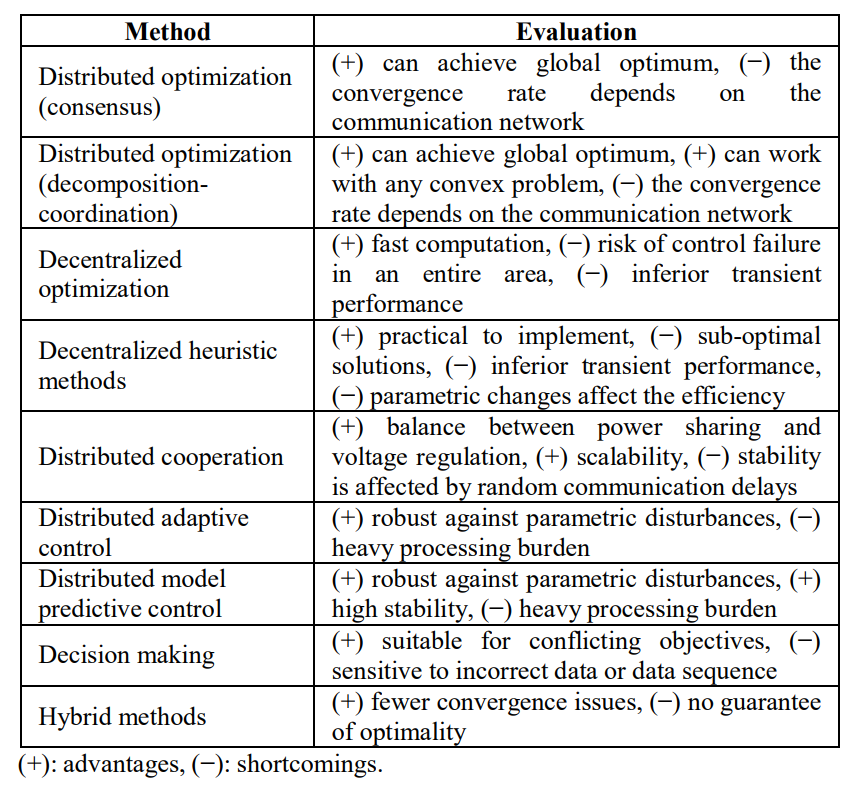
\includegraphics[width=0.85\linewidth]{figs/DIS_CVC.png}
\caption[Evaluation of mentioned methods]{Evaluation of mentioned methods \cite{Kyrue}}
\label{fig:DIS_CVC}
\end{figure}

\section{Energy Management}
With real-time pricing and variability of DGs, energy management can play a vital role to decrease the cost of energy. The goal of a modern energy management system would be to optimize the use of energy storage not only based on the current state of the system but also based on the probable future states. The energy management algorithms which deal with both variable DGs and real-time pricing can be divided into two main categories, offline and real-time algorithms \cite{Wen17}. 
\subsection{Offline Algorithms}
The offline optimization algorithms usually optimize energy for a predetermined time horizon based on prediction data. Researchers in \cite{ACh13} use neural network combined with linear programming based multi-objective optimization to optimize the use of several DERs in a microgrid. They also use fuzzy logic based expert system to schedule the use of energy storage. Fig. \ref{fig:OFF_1} shows the microgrid architecture under consideration in this research. The researchers use 24-hour ahead PV forecasting and 1-hour ahead wind energy forecasting to optimize the use of the resources. Although this approach guarantees global optimization, huge computation power is necessary to scale this for larger systems. Also, the optimality of the solution is based on considering perfect prediction.

\begin{figure}[!h]
\centering
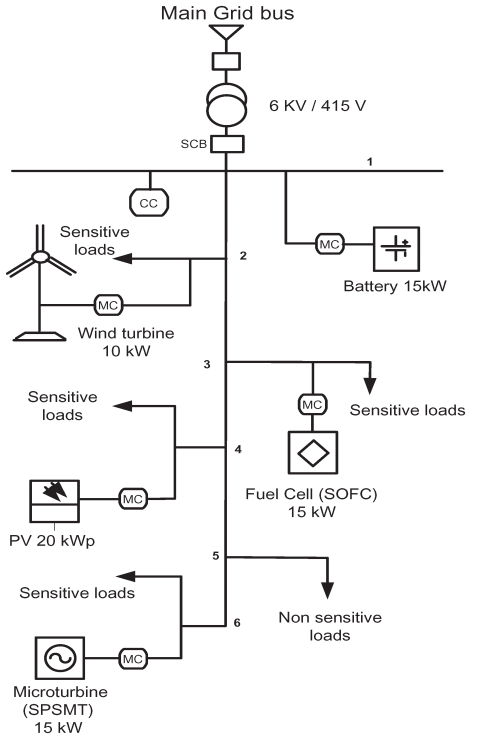
\includegraphics[width=0.5\linewidth, angle = 90]{figs/OFF_1.png}
\caption[Microgrid architecture under consideration]{Microgrid architecture under consideration in \cite{ACh13}.}
\label{fig:OFF_1}
\end{figure}

Researchers in \cite{AKh14} propose a microgrid optimization problem which runs the microgrid in islanded mode if enough generation is available and connects to the grid if enough generation is not available in the microgrid or the cost of using the local DERs becomes higher than the grid cost. Fig. \ref{fig:OFF_2}  shows the flowchart of the proposed scheduling model. The problem is defined in two parts. A grid-connected operation master problem a subproblem for islanded operation. First, the master problem determines the optimal scheduling of the available resources with the grid. Then the schedule is passed down to the subproblem to determine the feasibility of the microgrid operation. If the microgrid does not have the capability to pertain to the schedule, it cuts back the deficiencies from the schedule and returns the new schedule to the main problem.  The proposed method schedules the microgrid operation intentional islanding operations a day ahead based on predicted data. This makes the method highly reliant on perfect prediction. \cite{WSh15} presents an off-line method that takes into account the underlying structure of the grid. The researchers propose a scheduling method based on optimum power flow to ensure none of the scheduled states violate system constraints. The system is optimally scheduled taking the help of both a global controller and locally placed distributed controllers. The methods mentioned thus far show significant saving under ideal conditions. However, the reliability on perfect prediction and non-scalable nature of some of the solutions make them impractical for implementation on the actual grid.

\begin{figure}[!h]
\centering
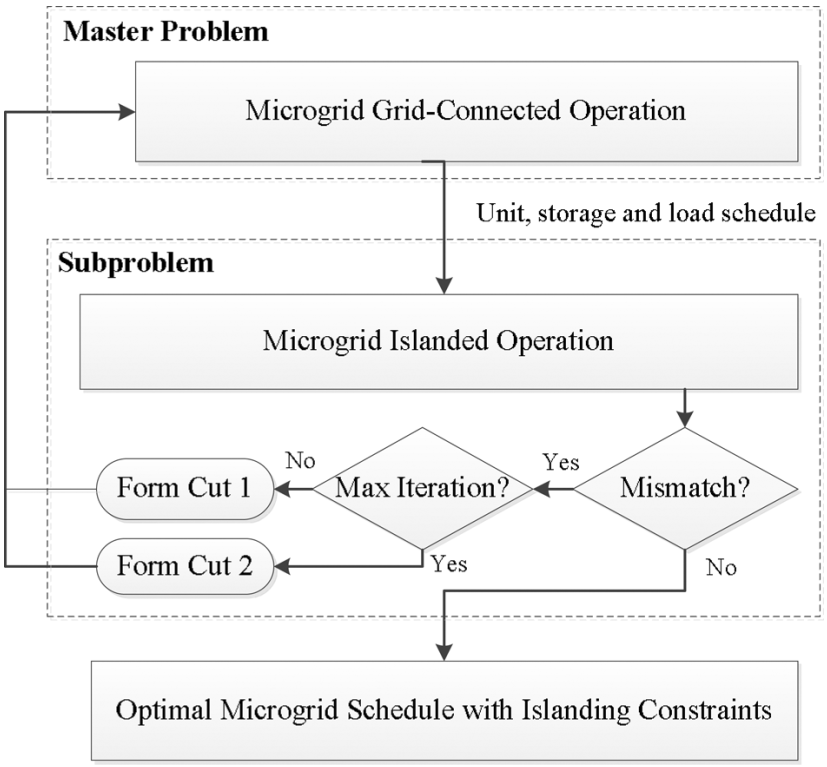
\includegraphics[width=0.5\linewidth]{figs/OFF_2.png}
\caption[Proposed scheduling model]{Proposed scheduling model  in \cite{AKh14}.}
\label{fig:OFF_2}
\end{figure}

To solve the problem of reliance on perfect prediction some offline algorithms, try to model the uncertainties in day-ahead scheduling and try to develop optimum schedules taking into account the probable uncertainties.
\cite{Has17} uses mixed integer linear programming formulation of the day ahead scheduling of microgrids. The uncertainties are taken into account by calculating multiple solutions based on different predicted seniors. 
The authors in \cite{Yue16} formulate the optimization problem based on the worst case scenario. The solution method considers the most cost from the grid and the least benefits from using local DG resources. The uncertainty of the grid is expressed as set points in Taguchi’s orthogonal array. Then search strategy based on Taguchi’s orthogonal array is used to find the best possible solution cases. Using the worst case to formulate the problem makes the solution robust for all situations. Although this method provides a robust solution always taking into account, the worst scenario makes the solution suboptimal.
\cite{FFa15} uses the mixed inter programming formulation for optimizing the DERs. The uncertainties of the predicted data are taken into account by generating different schedules with risk-averse and risk-neutral options. The different scenarios are stochastically generated based on the risk-based prediction data available. The approach uses stochastic programming to generate the uncertainties as different scenarios. The number of scenarios required to adequately capture the uncertainties usually end up being very large. 





\subsection{Real-Time Algorithms}
There have been advances recently in designing real-time algorithms that optimize the long-term cost of the energy management system taking into account the intermittent nature of the loads and DGs in the grid. \cite{RPa13} Proposes a real-time management process based on a rolling horizon strategy. The algorithm proposed solves a mixed integer linear programming problem in each interval to generate set points for the resources available. The researchers test the algorithm using a microgrid model consisting of PV panel, diesel generator, wind turbine and energy storage system. Fig. \ref{fig:RT_1} shows a block diagram of the proposed method As it can be seen from the diagram the method takes into account historical data, current measurement and weather forecast in the optimization process. The system discussed has to solve a mixed integer linear program on every time interval. This process is computationally intensive and becomes exponentially more complex with the addition of more energy resources.
\begin{figure}[!h]
\centering
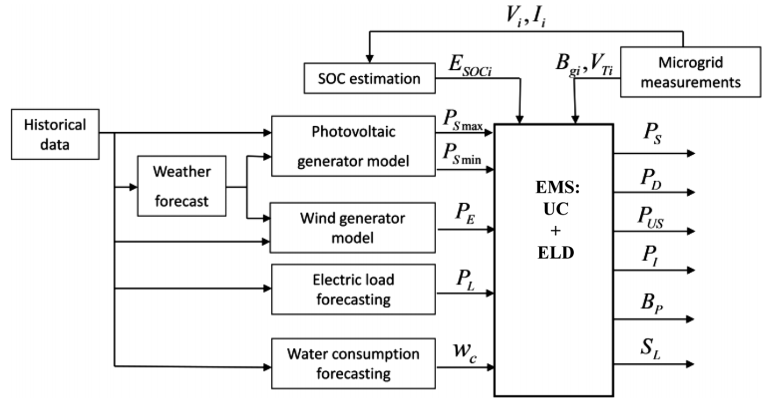
\includegraphics[width=0.85\linewidth]{figs/RT_1.png}
\caption[A block diagram of proposed energy management system]{A block diagram of proposed energy management system  \cite{RPa13}.}
\label{fig:RT_1}
\end{figure}

 Researchers in \cite{Sun14} use an aggregator to minimize the long-term cost of the grid. Figure 40 shows the top level schematic representation of the control architecture proposed. The solution used Lyapunov optimization to solve the energy management problem in real-time. The method proposed does not consider the actual architecture of the grid and optimizes considering all the components are connected to the same bus. This makes it impractical due to the actual grid having line constraints that cannot be violated.

\begin{figure}[!h]
\centering
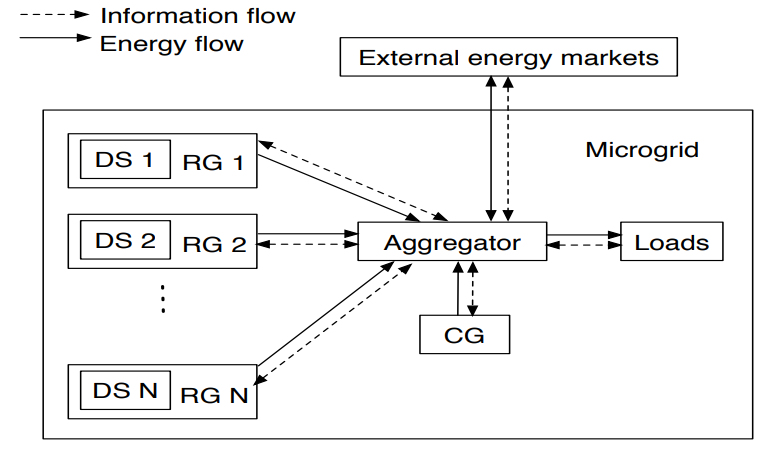
\includegraphics[width=0.85\linewidth]{figs/RT_2.png}
\caption[Schematic representation of solution method prepossessed]{Schematic representation of solution method prepossessed in \cite{Sun14}.}
\label{fig:RT_2}
\end{figure}

\cite{Men16} formulates the problem as a real-time one leader N-follower Stackelberg game and shows an efficient approach designed to optimize the system based on a demand response scheme. The optimization is performed by creating a virtual electricity trading market where the facility (leader) produces virtual prices of electricity and the resources (followers) compete to buy and sell electricity. The researchers show the existence of unique Stackelberg equilibrium for optimum use of each resource.

In \cite{Tia17}, researchers propose a multi-period AC optimal power flow taking into account the uncertainties of the solar and wind resources to ensure reliable solutions for the distribution system operators. Figure 41 shows the developed method in \cite{Tia17}. In the first stage the algorithm contacts with all the available resources to determine the upper and lower bounds of generation throughout the next day. The upper and lower bounds of the different units are termed as flexibility in the paper. In the second stage which is the real-time operation, the algorithm optimizes in real-time taking into account the flexibility of the available resources. 
 
\begin{figure}[!h]
\centering
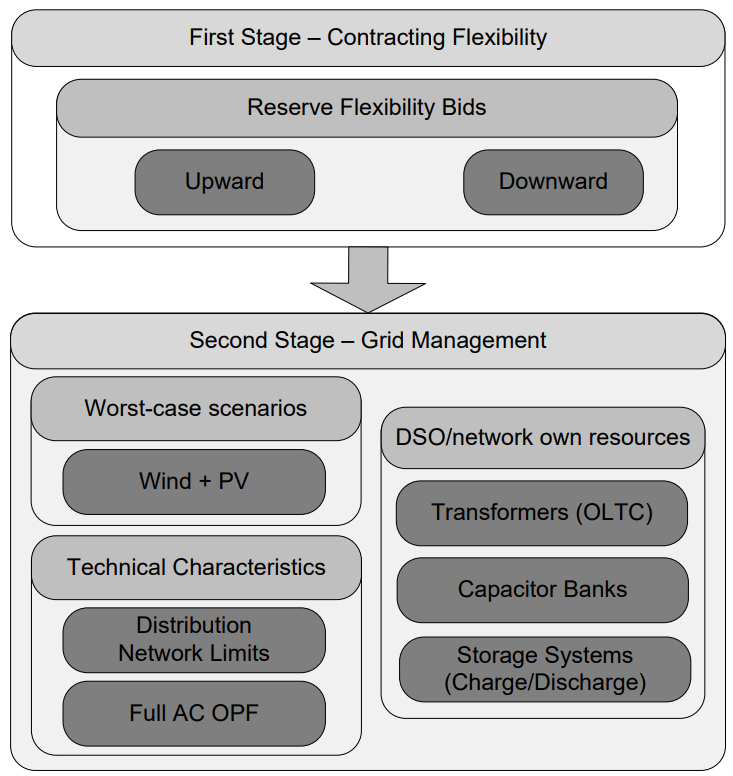
\includegraphics[width=0.5\linewidth]{figs/RT_3.png}
\caption[Methodology developed]{Methodology developed in \cite{Tia17}.}
\label{fig:RT_3}
\end{figure}

\cite{Wen17} proposes to solve the problem using an online energy management system in real-time using Lyapunov optimization taking into account the physical constraints of the system.
The drawbacks of these methods are that most of them do not take into account the actual distribution system architecture while formulating the problem. Only \cite{Wen17} considers system architecture while optimizing in real-time. However, a lack of prediction based elements makes these methods optimal for short term costs but suboptimal for properly optimizing long term operating cost.


\section{Protection}
The traditional protection devices available in the distribution network are circuit breakers, reclosers, sectionalizes and fuses. The traditional grid protection is coordinated using inverse definite minimum time (IDMT) curves. These curves are used to rate the protection devices to protect against over current and earth faults. The IDMT based solutions were optimized to make sure minimum number of customers were affected by the faults. The traditional network had only one source of fault current. So the IDMT based solutions did not take into account the effects of DERs. These protection schemes have been shown to be insufficient with a high DG penetration in \cite{PR133} and \cite{PR134}. The IEEE Standard 1547-2003 states that
“Any distributed resource installation connected to a spot network shall not cause operation or prevent reclosing of any network protectors installed on the spot network. This coordination shall be accomplished without requiring any changes to prevailing network protector clearing time practices of the area electric power system \cite{PR135}.” 
So according to the current standards there should be a maximum limit to DG integration in the system. There is research going on to determine the specific boundary of DG integration without altering the traditional protection scheme \cite{PR136}. 
From the research presented in \cite{PR137} it is evident that if we want to increase DG penetration in the distribution system we need to change our protection system to counter the effects of DG integration. One existing protection scheme that may be implemented to tackle these issues is the over current (OC) protection relay with directional elements. This technology is quite mature as has been used in the traditional distribution system \cite{PR137}. Unlike the traditional distribution system, the transmission system always had multiple sources feeding into it. And in theory, the directional OC protection scheme implemented in transmission systems can be a viable solution for the distribution grid. This method of protection is proposed in \cite{PR138}. The authors of  \cite{PR138} propose that  a DER connected in the middle of a distribution line should have directional protection devices on each side of the point of common coupling (PCC). There are many drawbacks to this proposal. Firstly, the method proposed will require two directional protection relays for each DER connected to the grid. It would be very costly. They also assume that the DERs are interfaced through synchronous units. The DERs interfaced with power electronics may not produce enough fault current to trip the protection system.  Moreover, the non-directional protection connected at the beginning of the feeder may trip due to fault in a neighboring feeder  \cite{PR137}.
 In \cite{PR139} Choi J. et al. propose an adaptive protection scheme. The proposed protection scheme used OC and voltage based methods for fault detection. Threshold values of ‘critical current’ and ‘critical voltage’ are defined for PCC of the Dg units. These critical values are used in case of faults within the inter-tie circuit breaker zone. If the relay detects these critical values within the inter-tie circuit breaker zone an instantaneous trip occurs. Otherwise, the IDMT curve based protection scheme is used. The protection scheme proposed can be inadequate for high impedance faults caused by inverter interfaced DGs. The distribution lines may cover large areas and substation voltage drops may be frequent \cite{PR137}. This would likely cause the voltage based protection at PCC to trip due to a voltage regulation issue not related to actual faults in the system. there might also be complications detecting phase to ground faults as earthing connection and transformer connection can prevent the flow of zero sequence fault current flow at the PCC.
A distance protection based solution is proposed in \cite{PR140}. Distance protection is directional, and this property makes it suitable for non-radial networks. The authors in \cite{PR140} propose connecting distance protection on the low voltage side of the distribution transformer to avoid the cost of a voltage transformer. To tackle the issue of no measurable zero sequence current on the low voltage side due to a fault on the high voltage side of the transformer, the scheme proposes using a preset estimate of the impedance behind the distance relay during phase-to-earth faults. Although this research in \cite{PR140} shows good potential for distance protection methods, more research is needed to properly determine the preset estimates.
The authors in \cite{PR140} propose another OC protection scheme with the help of a central controller. This scheme is only viable in systems that do not have inverter interfaced DER.
A protection scheme for inverter interfaced DER is proposed in \cite{PR142}. The authors in \cite{PR142} use the sequence currents to detect faults. Then it uses time delays to achieve protection coordination. The implementation of this method requires a fault current limiter. The drawbacks of the proposed method are discrimination capabilities. The zero sequence current during a high impedance fault might be similar to unbalanced load current. The scheme also does not take into account the possibility of transformer configuration and earthing paths may provide multiple or no zero sequence current paths.
The authors in \cite{PR143} propose a negative sequence current based protection scheme. And for high impedance fault, the method proposed in \cite{PR144} is incorporated. This method uses blocking signals to ensure selectivity in fault and it also provides backup protection for circuit breakers. The proposed method performs optimally with proper communication. But it can also perform sub optimally if there is a communication failure. The tradeoff would be that if there is a communication failure the method will disconnect more consumers than necessary. 
A differential energy based scheme is presented in  \cite{PR145}. The current at each protection device is converted to spectral energy content using S-transform. The spectral energy using the data gathered at the opposite end is then calculated. These results are used to calculate the differential spectral energy. This proposed scheme is reliant on communication and there is no backup suggested in case of communication failure. 
Another protection scheme based on differential current and symmetrical current components is proposed in \cite{PR146}. The protection scheme proposed is proven to effectively determine phase to earth and line to line faults. The authors propose the use of zero and negative sequence currents to identify the faults. They take into account the unbalanced loading conditions and coordinate protection settings for the relays. They are tuned in such a way that a tripping will not occur during the extremes of unbalanced conditions and a trip should occur if there is a high impedance fault in the relay’s protection zone.




\section{Research Gap}
From the discussion thus far it is evident that there are still many research opportunities in the field of coordinated voltage control and real-time energy management of distribution grids containing DERs. Some of the research gaps in literature are:

\begin{itemize}
    \item Coordinated voltage control research gap: The available solutions use the traditional regulation devices to regulate voltage. They use the available inverter interfaced DGs mostly as passive devices. Some of them use local volt-var optimization to maintain the voltage at the local node. But they do not globally coordinate the reactive power generation capabilities of the inverter interfaced DERs with the traditional regulation devices to optimal use of the available regulation potential. The global controls discussed in the literature are computationally intensive. There is also a lack of control schemes that optimizes the use of all available regulation devices and the DGs to tackle voltage violation.
    
    \item Real-time energy management research gap: With the increasing amount of variable DGs being added to the grid it is becoming very difficult to have accurate long term prediction of grid status. The presently available solutions either use present grid status to do real time control or use day ahead scheduling or use a mix of both to do energy management. There is still need of an energy management scheme that can optimize system status in real-time with a continuously updating forecast. 
\end{itemize}

\section{Contribution}
The efforts invested in the dissertation work at hand mainly aim towards the following:
 
\subsection{Development of coordinated voltage control algorithm}
A coordinated voltage control algorithm will be developed which can make use of the reactive power generation capabilities of the inverter interfaced DERs and coordinate these resources with the existing traditional regulation devices. For this purpose, a solution methodology combining the Voltage Sensitivity Analysis \cite{Th_ali} and Electrical Distance Calculation \cite{Alvi3} concepts will be explored.

Major work under this task:
\begin{itemize}
    \item Design of proposed voltage control algorithm 
    \item Implementation of voltage control model in centralized or decentralized network typologies
    \item Compare performance of proposed model with traditional voltage regulation scheme
\end{itemize}

\subsection{Development of real-time energy management system}
An energy management system that takes into account the physical system constraints while optimizing the use of available energy resources not only based on the current price but also based on the forecasted price will be developed. This part will be implemented by dividing the energy storage in separate states and creating a graph taking into account the system constraints. The solution of the energy management problem will be developed using a combination of the traditional optimal dispatch of generation solution, using the Linear programming model with DC power flow, with a graph search solution obtained from the utilization of the A* algorithm designed to find the optimal and most cost effective solution for dispatching available energy resources taking into account not only the present status of the system, but also the future forecasting values of the energy prices, load demand, and generation.
To accommodate the forecasted data into decision making. The energy storage (ES) capability of the system is divided into discrete states of charge (SOC). Then a graph is constructed to represent the states of charges with respect to time. Each edge of the graph will have a total cost. The total cost will be calculated taking into account the economic dispatch of the resources available in the system. After the graph is constructed A* search algorithm will be used to find the optimal path.

Major work under this task:
\begin{itemize}
    \item Design of proposed A* star algorithm model 
    \item Integration of forecasting information
    \item Compare performance of proposed model with other available schemes.
\end{itemize}


At present, a coordinated voltage control algorithm has been developed and validated using off-line simulation. Currently, it is assumed that the algorithm has access to the system voltage magnitude and angles. Moreover, a real-time energy management algorithm to optimize the use of a single grid-connected energy storage has been developed. The algorithm has been validated using controller hardware in the loop simulation.